% !TeX spellcheck = en_US
% !TeX encoding = UTF-8
\chapter{Theoretical foundation}

\section{Stress Measurement-Objective Measures}
\subsection{Photoplethysmogram-PPG}
\subsection{Electrodermal Activity-EDA}
\subsection{Empatica E4}
https://support.empatica.com/hc/en-us/articles/204954639-Utilizing-the-PPG-BVP-signal
https://support.empatica.com/hc/en-us/articles/360029719792-E4-data-BVP-expected-signal
%https://box.empatica.com/documentation/20141119_E4_TechSpecs.pdf

\subsection{Motion Capture}
\begin{figure}[h]
    \centering
    % First image
    \begin{subfigure}[b]{0.45\columnwidth}
        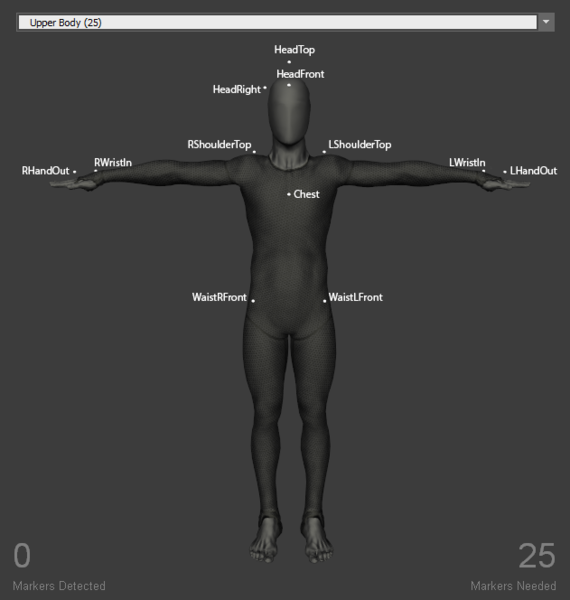
\includegraphics[width=\textwidth]{images/skleton.png}
        \caption{Front View }
        \label{fig:phone1}
    \end{subfigure}
    % Second image
    \begin{subfigure}[b]{0.45\columnwidth}
        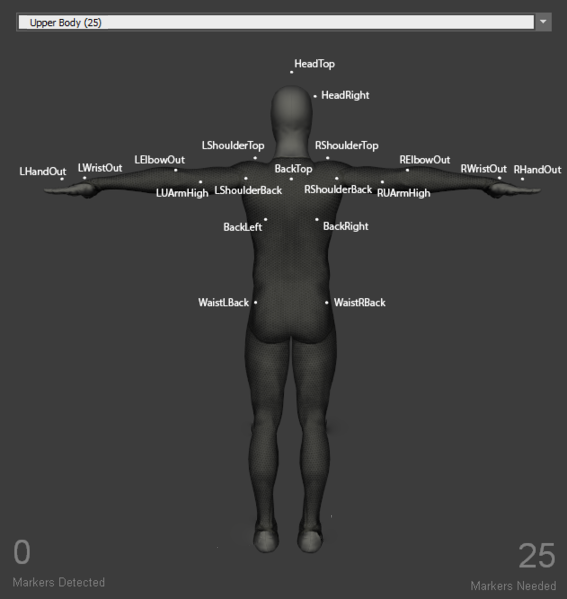
\includegraphics[width=\textwidth]{images/skeleton2.png}
        \caption{Back View }
        \label{fig:phone2}
    \end{subfigure}
    \caption{25 Upper Body Marker Set}
    \label{fig:phone}
\end{figure}

\section{Subjective Measures}
Mental stress can be assessed through subjective and objective
measures. Subjective ratings, such as self-report questionnaires, have
been commonly used to estimate levels of mental stress in humans
(Aigrain et al., 2018). Participants are asked to answer a variety of
questions about their experiences in the experiment. The NASA-Task
Load Index (NASA-TLX) has been utilized in numerous research
studies to assess people’s mental stress levels. For instance, Zheng et al.
(2012) employed the NASA-TLX to investigate the mental workload
experienced by surgeons during endoscopy training. In the context of
smart factories, Zakeri et al. (2021) applied the NASA-TLX to examine
various factors contributing to mental stress, such as task complexity,
time constraints, and collaboration duration. However, it is important to
acknowledge the limitations of self-reporting, as participants cannot
report in real-time and may not express their true feelings (Bethel et al.,
2007). 

\section{Devices Used}
Should it be added here or in the Experimental procedure. Some info on how th empatica and motion capture works.
\section{UR10 robot and collsion avoidance }


